%%%%%%%%%%%%%%%%%%%%%%%%%%%%%%%%%%%%%%%%%
% Algorithm Visualization Automation
% Poster Presentation
%
% Template created by:
% Computational Physics and Biophysics Group, Jacobs University
% https://teamwork.jacobs-university.de:8443/confluence/display/CoPandBiG/LaTeX+Poster
% 
% Template further modified by:
% Nathaniel Johnston (nathaniel@njohnston.ca)
% 
% Poster presentation adapted by:
% Michael Galliers (KYDronePilot)
%
% License:
% CC BY-NC-SA 3.0 (http://creativecommons.org/licenses/by-nc-sa/3.0/)
%
%%%%%%%%%%%%%%%%%%%%%%%%%%%%%%%%%%%%%%%%%

%----------------------------------------------------------------------------------------
%	PACKAGES AND OTHER DOCUMENT CONFIGURATIONS
%----------------------------------------------------------------------------------------

\documentclass[final]{beamer}

\usepackage[scale=1.24]{beamerposter} % Use the beamerposter package for the poster

\usepackage{forest} % For rendering the decision trees

\usepackage{pdfpages} % For includng pre-rendered decision trees

\usetheme{confposter} % Use the confposter theme supplied with this template

\setbeamercolor{block title}{fg=ngreen,bg=white} % Colors of the block titles
\setbeamercolor{block body}{fg=black,bg=white} % Colors of the body of blocks
% Colors of the highlighted block titles
\setbeamercolor{block alerted title}{fg=white,bg=dblue!70}
% Colors of the body of highlighted blocks
\setbeamercolor{block alerted body}{fg=black,bg=dblue!10}
% Many more colors are available for use in beamerthemeconfposter.sty

%-----------------------------------------------------------
% Define the column widths and overall poster size
% To set effective sepwid, onecolwid and twocolwid values, first choose how many columns
% you want and how much separation you want between columns
% In this template, the separation width chosen is 0.024 of the paper width and a
% 4-column layout
% onecolwid should therefore be (1-(# of columns+1)*sepwid)/# of columns e.g.
% (1-(4+1)*0.024)/4 = 0.22
% Set twocolwid to be (2*onecolwid)+sepwid = 0.464
% Set threecolwid to be (3*onecolwid)+2*sepwid = 0.708

\newlength{\sepwid}
\newlength{\onecolwid}
\newlength{\twocolwid}
\newlength{\threecolwid}
\setlength{\paperwidth}{48in} % A0 width: 46.8in
\setlength{\paperheight}{36in} % A0 height: 33.1in
\setlength{\sepwid}{0.024\paperwidth} % Separation width (white space) between columns
\setlength{\onecolwid}{0.22\paperwidth} % Width of one column
\setlength{\twocolwid}{0.464\paperwidth} % Width of two columns
\setlength{\threecolwid}{0.708\paperwidth} % Width of three columns
\setlength{\topmargin}{-0.7in} % Reduce the top margin size

% Set up the column width for the three sub-columns in the middle column
\newlength{\onecolwidmid}
\setlength{\onecolwidmid}{0.1467\paperwidth}

%-----------------------------------------------------------

\usepackage{graphicx}  % Required for including images

\usepackage{booktabs} % Top and bottom rules for tables

%----------------------------------------------------------------------------------------
%	TITLE SECTION 
%----------------------------------------------------------------------------------------

\title{Algorithm Visualization Automation} % Poster title

\author{Michael Galliers} % Author

\institute{Eastern Kentucky University - Department of Computer Science} % Institution

%----------------------------------------------------------------------------------------

\begin{document}

\addtobeamertemplate{block end}{}{\vspace*{2ex}} % White space under blocks
% White space under highlighted (alert) blocks
\addtobeamertemplate{block alerted end}{}{\vspace*{2ex}}

\setlength{\belowcaptionskip}{2ex} % White space under figures
\setlength\belowdisplayshortskip{2ex} % White space under equations

\begin{frame}[t] % The whole poster is enclosed in one beamer frame

% The whole poster consists of three major columns, the second of which is split into two
% columns twice - the [t] option aligns each column's content to the top
\begin{columns}[t]

\begin{column}{\sepwid}\end{column} % Empty spacer column

\begin{column}{\onecolwid} % The first column

%----------------------------------------------------------------------------------------
%	INTRODUCTION
%----------------------------------------------------------------------------------------

\begin{block}{Introduction}

Computer algorithms are the basis for how computers solve problems. Algorithms describe the series
of steps a program must take to complete a certain task. This includes checking conditions and
performing actions based on those conditions. Having the ability to visualize how algorithms operate
while designing them can be extremely valuable. Automation of the visualization process can be even
more useful in development, quickly showing ways in which algorithms could be improved to increase
efficiency.

\end{block}

%----------------------------------------------------------------------------------------
%	SORTING ALGORITHMS
%----------------------------------------------------------------------------------------

\begin{block}{Sorting Algorithms}

Sorting is a heavily studied topic in computer science. Many types of sorting algorithms have been
developed and each has its advantages and disadvantages. \textit{\textbf{Bubble Sort}} is one of the
most basic. It works by comparing the first 2 elements in a list and swapping them if the first is
greater than the second. This repeats with the second and third elements and so on until the
greatest element is \textit{bubbled} to the last position. The process is repeated to
\textit{bubble} the second greatest element to behind the greatest, and so on until the list is
sorted.

\end{block}

%----------------------------------------------------------------------------------------
%	DECISION TREES
%----------------------------------------------------------------------------------------

\begin{block}{Decision Trees}

In algorithm analysis, a \textbf {pruned decision tree} is a tree that describes all possible
execution paths a program can take, depending on the input, with any contradictory paths
\textit{pruned}. For sorting algorithms, this tree is \textbf{valid} if there is a path from the
root node to a leaf node that sorts any permutation of an inputted list \cite{neapolitan:2015}. A
\textbf{pruned- valid decision tree} can be interpreted as the different execution paths a program
can take and the efficiency of each path. The fewer nodes in a path from the root to a leaf node,
the less comparisons performed, and the more efficient the algorithm.

\end{block}

%----------------------------------------------------------------------------------------

\end{column} % End of the first column

\begin{column}{\sepwid}\end{column} % Empty spacer column

\begin{column}{\twocolwid} % Begin a column which is two columns wide (column 2)

%----------------------------------------------------------------------------------------
%	BUBBLE SORT TREE
%----------------------------------------------------------------------------------------

\begin{figure}
% 
\includegraphics[width=0.8\linewidth]{figures/bubble_sort_4_elements.png}
\resizebox{0.9\linewidth}{!}{\begin{forest}
  for tree={
    edge label = {font=\scriptsize},
    circle,
    draw,
    if n children=0{
      rectangle, draw
    }{}
  }
  [ $a > b$, edge label={node[midway,fill=white,font=\tiny] {}}
    [ $a > c$, edge label={node[midway,fill=white,font=\tiny] {Yes}}
      [ $a > d$, edge label={node[midway,fill=white,font=\tiny] {Yes}}
        [ $b > c$, edge label={node[midway,fill=white,font=\tiny] {Yes}}
          [ $b > d$, edge label={node[midway,fill=white,font=\tiny] {Yes}}
            [ $c > d$, edge label={node[midway,fill=white,font=\tiny] {Yes}}
              [ d c b a, edge label={node[midway,fill=white,font=\tiny] {Yes}} ]
              [ c d b a, edge label={node[midway,fill=white,font=\tiny] {No}} ]
            ]
            [ $c > b$, edge label={node[midway,fill=white,font=\tiny] {No}}
              [ , phantom ]
              [ c b d a, edge label={node[midway,fill=white,font=\tiny] {No}} ]
            ]
          ]
          [ $c > d$, edge label={node[midway,fill=white,font=\tiny] {No}}
            [ $b > d$, edge label={node[midway,fill=white,font=\tiny] {Yes}}
              [ d b c a, edge label={node[midway,fill=white,font=\tiny] {Yes}} ]
              [ b d c a, edge label={node[midway,fill=white,font=\tiny] {No}} ]
            ]
            [ $b > c$, edge label={node[midway,fill=white,font=\tiny] {No}}
              [ , phantom ]
              [ b c d a, edge label={node[midway,fill=white,font=\tiny] {No}} ]
            ]
          ]
        ]
        [ $b > c$, edge label={node[midway,fill=white,font=\tiny] {No}}
          [ $b > a$, edge label={node[midway,fill=white,font=\tiny] {Yes}}
            [ , phantom ]
            [ $c > b$, edge label={node[midway,fill=white,font=\tiny] {No}}
              [ , phantom ]
              [ c b a d, edge label={node[midway,fill=white,font=\tiny] {No}} ]
            ]
          ]
          [ $c > a$, edge label={node[midway,fill=white,font=\tiny] {No}}
            [ , phantom ]
            [ $b > c$, edge label={node[midway,fill=white,font=\tiny] {No}}
              [ , phantom ]
              [ b c a d, edge label={node[midway,fill=white,font=\tiny] {No}} ]
            ]
          ]
        ]
      ]
      [ $c > d$, edge label={node[midway,fill=white,font=\tiny] {No}}
        [ $b > a$, edge label={node[midway,fill=white,font=\tiny] {Yes}}
          [ , phantom ]
          [ $a > d$, edge label={node[midway,fill=white,font=\tiny] {No}}
            [ $b > d$, edge label={node[midway,fill=white,font=\tiny] {Yes}}
              [ d b a c, edge label={node[midway,fill=white,font=\tiny] {Yes}} ]
              [ b d a c, edge label={node[midway,fill=white,font=\tiny] {No}} ]
            ]
            [ $b > a$, edge label={node[midway,fill=white,font=\tiny] {No}}
              [ , phantom ]
              [ b a d c, edge label={node[midway,fill=white,font=\tiny] {No}} ]
            ]
          ]
        ]
        [ $b > a$, edge label={node[midway,fill=white,font=\tiny] {No}}
          [ , phantom ]
          [ $a > c$, edge label={node[midway,fill=white,font=\tiny] {No}}
            [ , phantom ]
            [ $b > a$, edge label={node[midway,fill=white,font=\tiny] {No}}
              [ , phantom ]
              [ b a c d, edge label={node[midway,fill=white,font=\tiny] {No}} ]
            ]
          ]
        ]
      ]
    ]
    [ $b > c$, edge label={node[midway,fill=white,font=\tiny] {No}}
      [ $b > d$, edge label={node[midway,fill=white,font=\tiny] {Yes}}
        [ $a > c$, edge label={node[midway,fill=white,font=\tiny] {Yes}}
          [ $a > d$, edge label={node[midway,fill=white,font=\tiny] {Yes}}
            [ $c > d$, edge label={node[midway,fill=white,font=\tiny] {Yes}}
              [ d c a b, edge label={node[midway,fill=white,font=\tiny] {Yes}} ]
              [ c d a b, edge label={node[midway,fill=white,font=\tiny] {No}} ]
            ]
            [ $c > a$, edge label={node[midway,fill=white,font=\tiny] {No}}
              [ , phantom ]
              [ c a d b, edge label={node[midway,fill=white,font=\tiny] {No}} ]
            ]
          ]
          [ $c > d$, edge label={node[midway,fill=white,font=\tiny] {No}}
            [ $a > d$, edge label={node[midway,fill=white,font=\tiny] {Yes}}
              [ d a c b, edge label={node[midway,fill=white,font=\tiny] {Yes}} ]
              [ a d c b, edge label={node[midway,fill=white,font=\tiny] {No}} ]
            ]
            [ $a > c$, edge label={node[midway,fill=white,font=\tiny] {No}}
              [ , phantom ]
              [ a c d b, edge label={node[midway,fill=white,font=\tiny] {No}} ]
            ]
          ]
        ]
        [ $a > c$, edge label={node[midway,fill=white,font=\tiny] {No}}
          [ $a > b$, edge label={node[midway,fill=white,font=\tiny] {Yes}}
            [ , phantom ]
            [ $c > a$, edge label={node[midway,fill=white,font=\tiny] {No}}
              [ , phantom ]
              [ c a b d, edge label={node[midway,fill=white,font=\tiny] {No}} ]
            ]
          ]
          [ $c > b$, edge label={node[midway,fill=white,font=\tiny] {No}}
            [ , phantom ]
            [ $a > c$, edge label={node[midway,fill=white,font=\tiny] {No}}
              [ , phantom ]
              [ a c b d, edge label={node[midway,fill=white,font=\tiny] {No}} ]
            ]
          ]
        ]
      ]
      [ $c > d$, edge label={node[midway,fill=white,font=\tiny] {No}}
        [ $a > b$, edge label={node[midway,fill=white,font=\tiny] {Yes}}
          [ , phantom ]
          [ $b > d$, edge label={node[midway,fill=white,font=\tiny] {No}}
            [ $a > d$, edge label={node[midway,fill=white,font=\tiny] {Yes}}
              [ d a b c, edge label={node[midway,fill=white,font=\tiny] {Yes}} ]
              [ a d b c, edge label={node[midway,fill=white,font=\tiny] {No}} ]
            ]
            [ $a > b$, edge label={node[midway,fill=white,font=\tiny] {No}}
              [ , phantom ]
              [ a b d c, edge label={node[midway,fill=white,font=\tiny] {No}} ]
            ]
          ]
        ]
        [ $a > b$, edge label={node[midway,fill=white,font=\tiny] {No}}
          [ , phantom ]
          [ $b > c$, edge label={node[midway,fill=white,font=\tiny] {No}}
            [ , phantom ]
            [ $a > b$, edge label={node[midway,fill=white,font=\tiny] {No}}
              [ , phantom ]
              [ a b c d, edge label={node[midway,fill=white,font=\tiny] {No}} ]
            ]
          ]
        ]
      ]
    ]
  ]
\end{forest}}
\caption{Bubble Sort on [$a$, $b$, $c$, $d$] - an inefficient sorting algorithm}
\end{figure}

%----------------------------------------------------------------------------------------

%----------------------------------------------------------------------------------------
%	INSERTION SORT TREE
%----------------------------------------------------------------------------------------

\begin{figure}
% 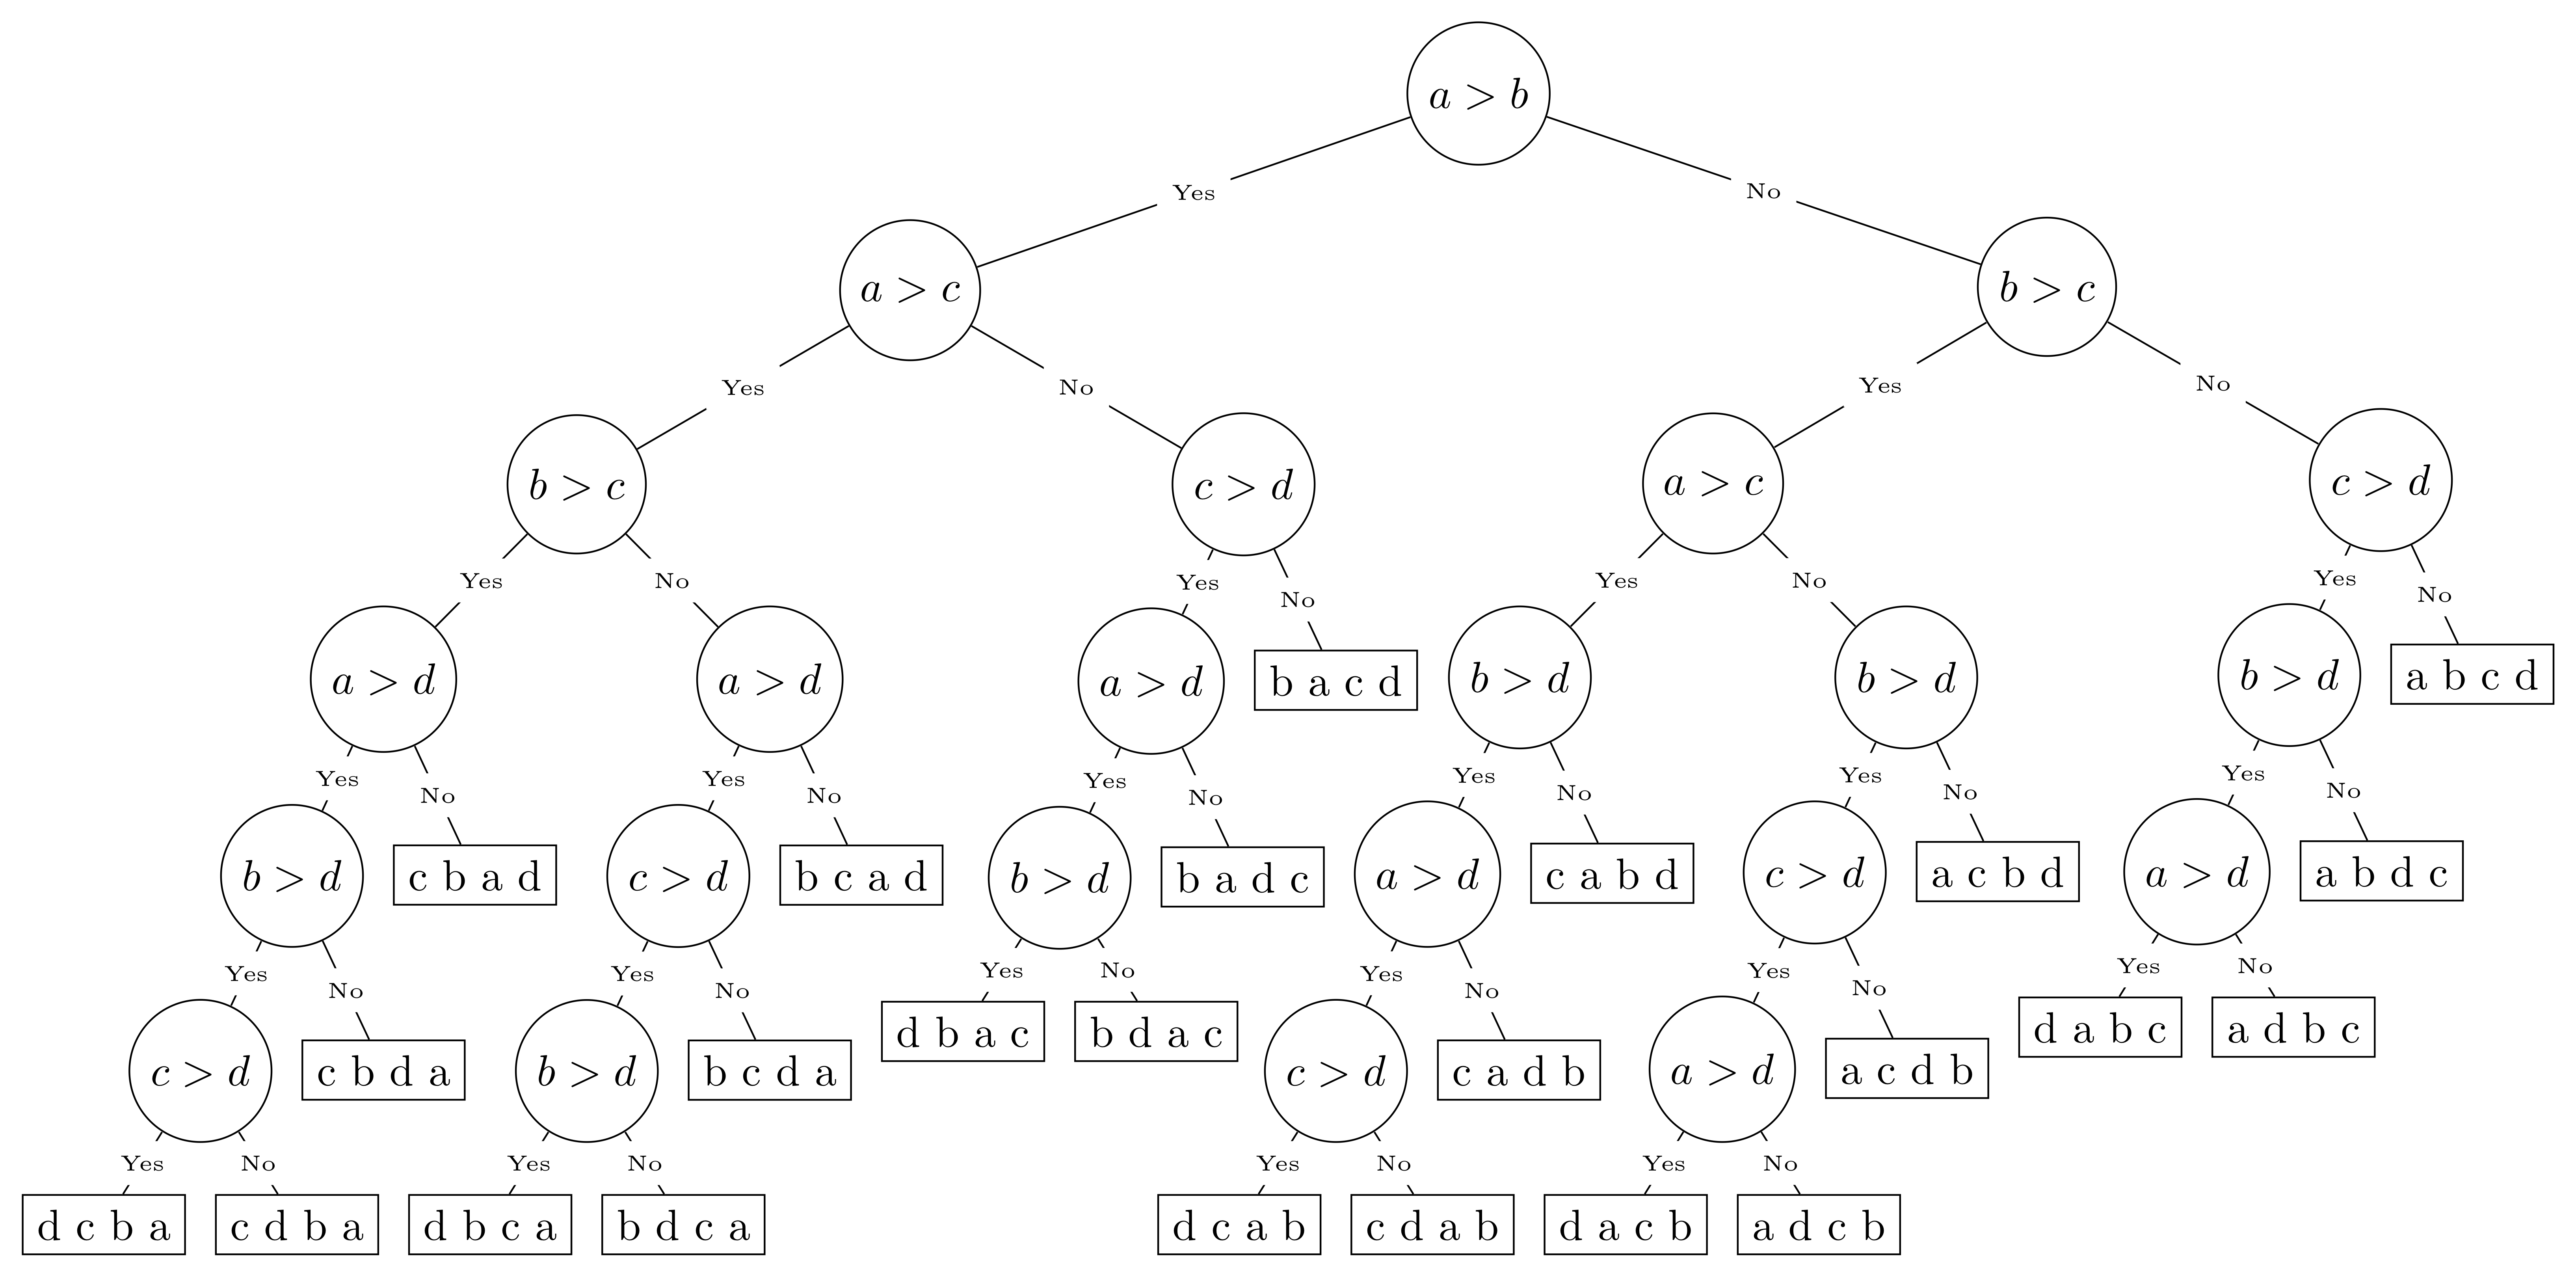
\includegraphics[width=0.8\linewidth]{figures/insertion_sort_4_elements.png}
\resizebox{0.9\linewidth}{!}{\begin{forest}
  for tree={
    edge label = {font=\scriptsize},
    circle,
    draw,
    if n children=0{
      rectangle, draw
    }{}
  }
  [ $a > b$, edge label={node[midway,fill=white,font=\tiny] {}}
    [ $a > c$, edge label={node[midway,fill=white,font=\tiny] {Yes}}
      [ $b > c$, edge label={node[midway,fill=white,font=\tiny] {Yes}}
        [ $a > d$, edge label={node[midway,fill=white,font=\tiny] {Yes}}
          [ $b > d$, edge label={node[midway,fill=white,font=\tiny] {Yes}}
            [ $c > d$, edge label={node[midway,fill=white,font=\tiny] {Yes}}
              [ d c b a, edge label={node[midway,fill=white,font=\tiny] {Yes}} ]
              [ c d b a, edge label={node[midway,fill=white,font=\tiny] {No}} ]
            ]
            [ c b d a, edge label={node[midway,fill=white,font=\tiny] {No}} ]
          ]
          [ c b a d, edge label={node[midway,fill=white,font=\tiny] {No}} ]
        ]
        [ $a > d$, edge label={node[midway,fill=white,font=\tiny] {No}}
          [ $c > d$, edge label={node[midway,fill=white,font=\tiny] {Yes}}
            [ $b > d$, edge label={node[midway,fill=white,font=\tiny] {Yes}}
              [ d b c a, edge label={node[midway,fill=white,font=\tiny] {Yes}} ]
              [ b d c a, edge label={node[midway,fill=white,font=\tiny] {No}} ]
            ]
            [ b c d a, edge label={node[midway,fill=white,font=\tiny] {No}} ]
          ]
          [ b c a d, edge label={node[midway,fill=white,font=\tiny] {No}} ]
        ]
      ]
      [ $c > d$, edge label={node[midway,fill=white,font=\tiny] {No}}
        [ $a > d$, edge label={node[midway,fill=white,font=\tiny] {Yes}}
          [ $b > d$, edge label={node[midway,fill=white,font=\tiny] {Yes}}
            [ d b a c, edge label={node[midway,fill=white,font=\tiny] {Yes}} ]
            [ b d a c, edge label={node[midway,fill=white,font=\tiny] {No}} ]
          ]
          [ b a d c, edge label={node[midway,fill=white,font=\tiny] {No}} ]
        ]
        [ b a c d, edge label={node[midway,fill=white,font=\tiny] {No}} ]
      ]
    ]
    [ $b > c$, edge label={node[midway,fill=white,font=\tiny] {No}}
      [ $a > c$, edge label={node[midway,fill=white,font=\tiny] {Yes}}
        [ $b > d$, edge label={node[midway,fill=white,font=\tiny] {Yes}}
          [ $a > d$, edge label={node[midway,fill=white,font=\tiny] {Yes}}
            [ $c > d$, edge label={node[midway,fill=white,font=\tiny] {Yes}}
              [ d c a b, edge label={node[midway,fill=white,font=\tiny] {Yes}} ]
              [ c d a b, edge label={node[midway,fill=white,font=\tiny] {No}} ]
            ]
            [ c a d b, edge label={node[midway,fill=white,font=\tiny] {No}} ]
          ]
          [ c a b d, edge label={node[midway,fill=white,font=\tiny] {No}} ]
        ]
        [ $b > d$, edge label={node[midway,fill=white,font=\tiny] {No}}
          [ $c > d$, edge label={node[midway,fill=white,font=\tiny] {Yes}}
            [ $a > d$, edge label={node[midway,fill=white,font=\tiny] {Yes}}
              [ d a c b, edge label={node[midway,fill=white,font=\tiny] {Yes}} ]
              [ a d c b, edge label={node[midway,fill=white,font=\tiny] {No}} ]
            ]
            [ a c d b, edge label={node[midway,fill=white,font=\tiny] {No}} ]
          ]
          [ a c b d, edge label={node[midway,fill=white,font=\tiny] {No}} ]
        ]
      ]
      [ $c > d$, edge label={node[midway,fill=white,font=\tiny] {No}}
        [ $b > d$, edge label={node[midway,fill=white,font=\tiny] {Yes}}
          [ $a > d$, edge label={node[midway,fill=white,font=\tiny] {Yes}}
            [ d a b c, edge label={node[midway,fill=white,font=\tiny] {Yes}} ]
            [ a d b c, edge label={node[midway,fill=white,font=\tiny] {No}} ]
          ]
          [ a b d c, edge label={node[midway,fill=white,font=\tiny] {No}} ]
        ]
        [ a b c d, edge label={node[midway,fill=white,font=\tiny] {No}} ]
      ]
    ]
  ]
\end{forest}}
\caption{Insertion Sort on [$a$, $b$, $c$, $d$] - a more efficient sorting algorithm}
\end{figure}

%----------------------------------------------------------------------------------------

\begin{columns}[t,totalwidth=\twocolwid] % Split up the two columns wide column again

\begin{column}{\onecolwidmid} % The first column within column 2 (column 2.1)

%----------------------------------------------------------------------------------------
%	ANALYZER STEP 1
%----------------------------------------------------------------------------------------

\begin{figure}
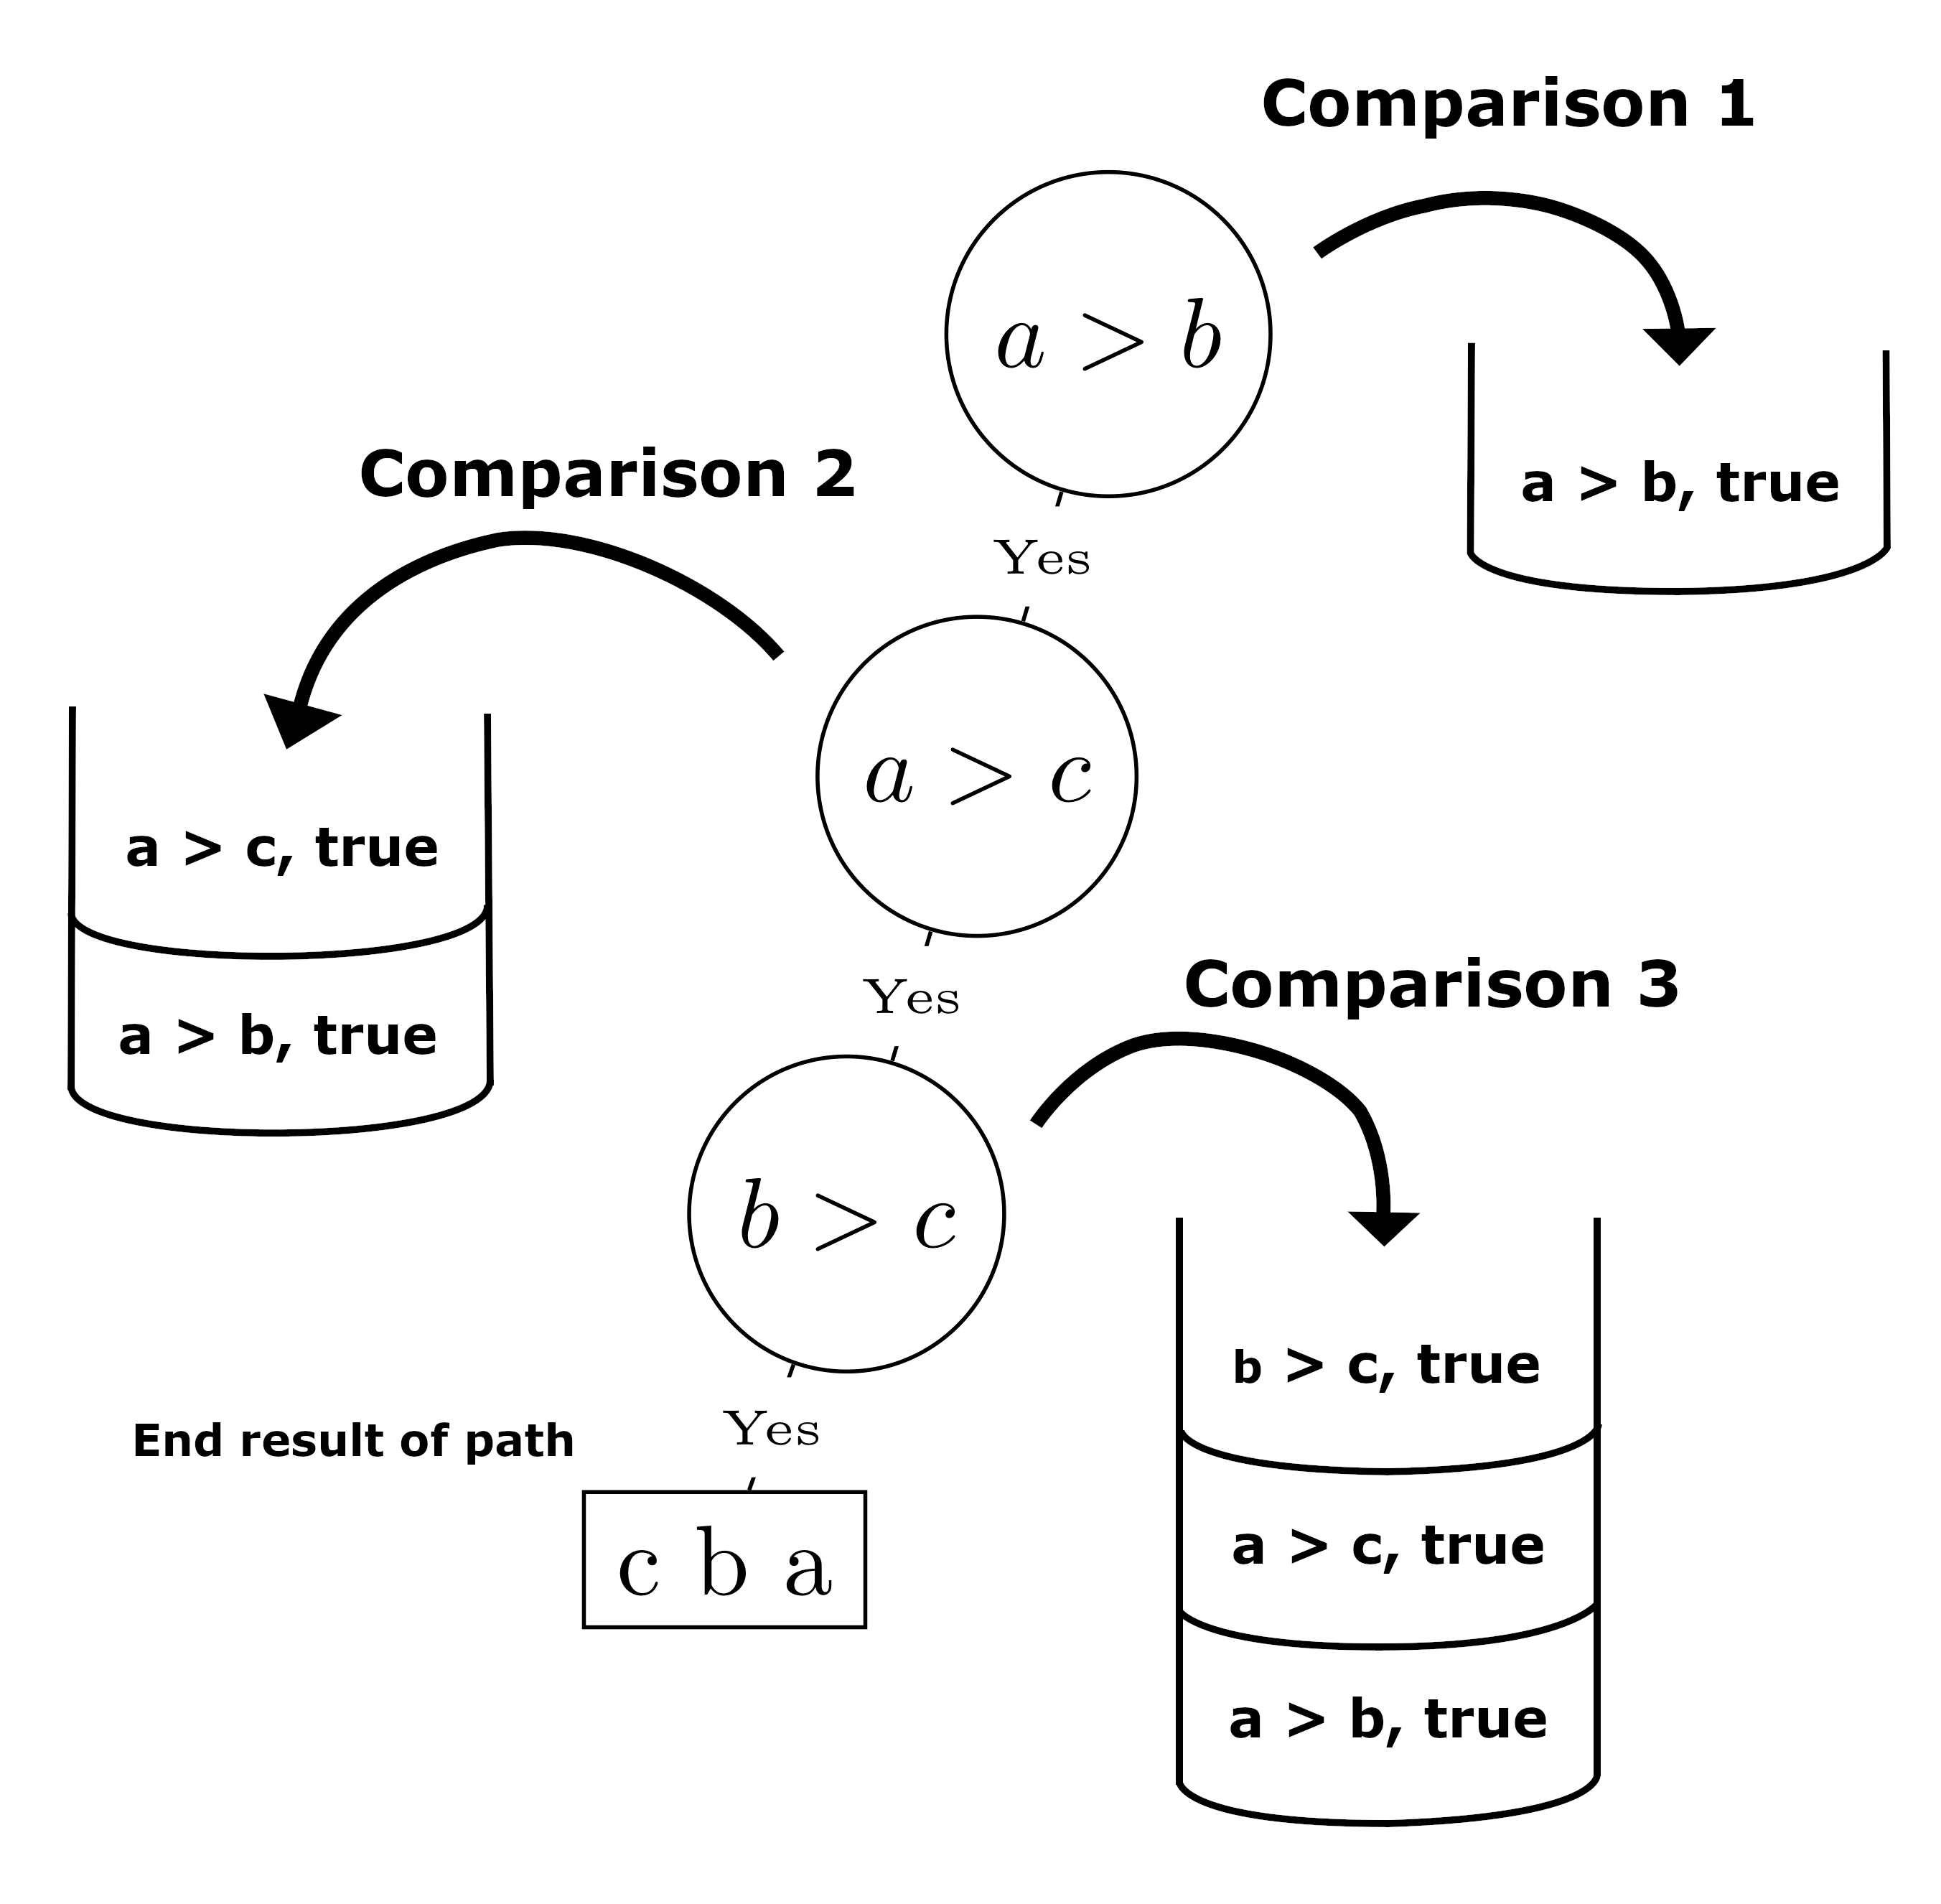
\includegraphics[width=0.8\linewidth]{figures/bubble_sort_step_1_formatted.png}
\caption{Analyzer Step 1 - Initial Traversal}
\label{analyzer:1}
\end{figure}

%----------------------------------------------------------------------------------------

\end{column} % End of column 2.1

\begin{column}{\onecolwidmid} % The second column within column 2 (column 2.2)

%----------------------------------------------------------------------------------------
%	ANALYZER STEP 2
%----------------------------------------------------------------------------------------

\begin{figure}
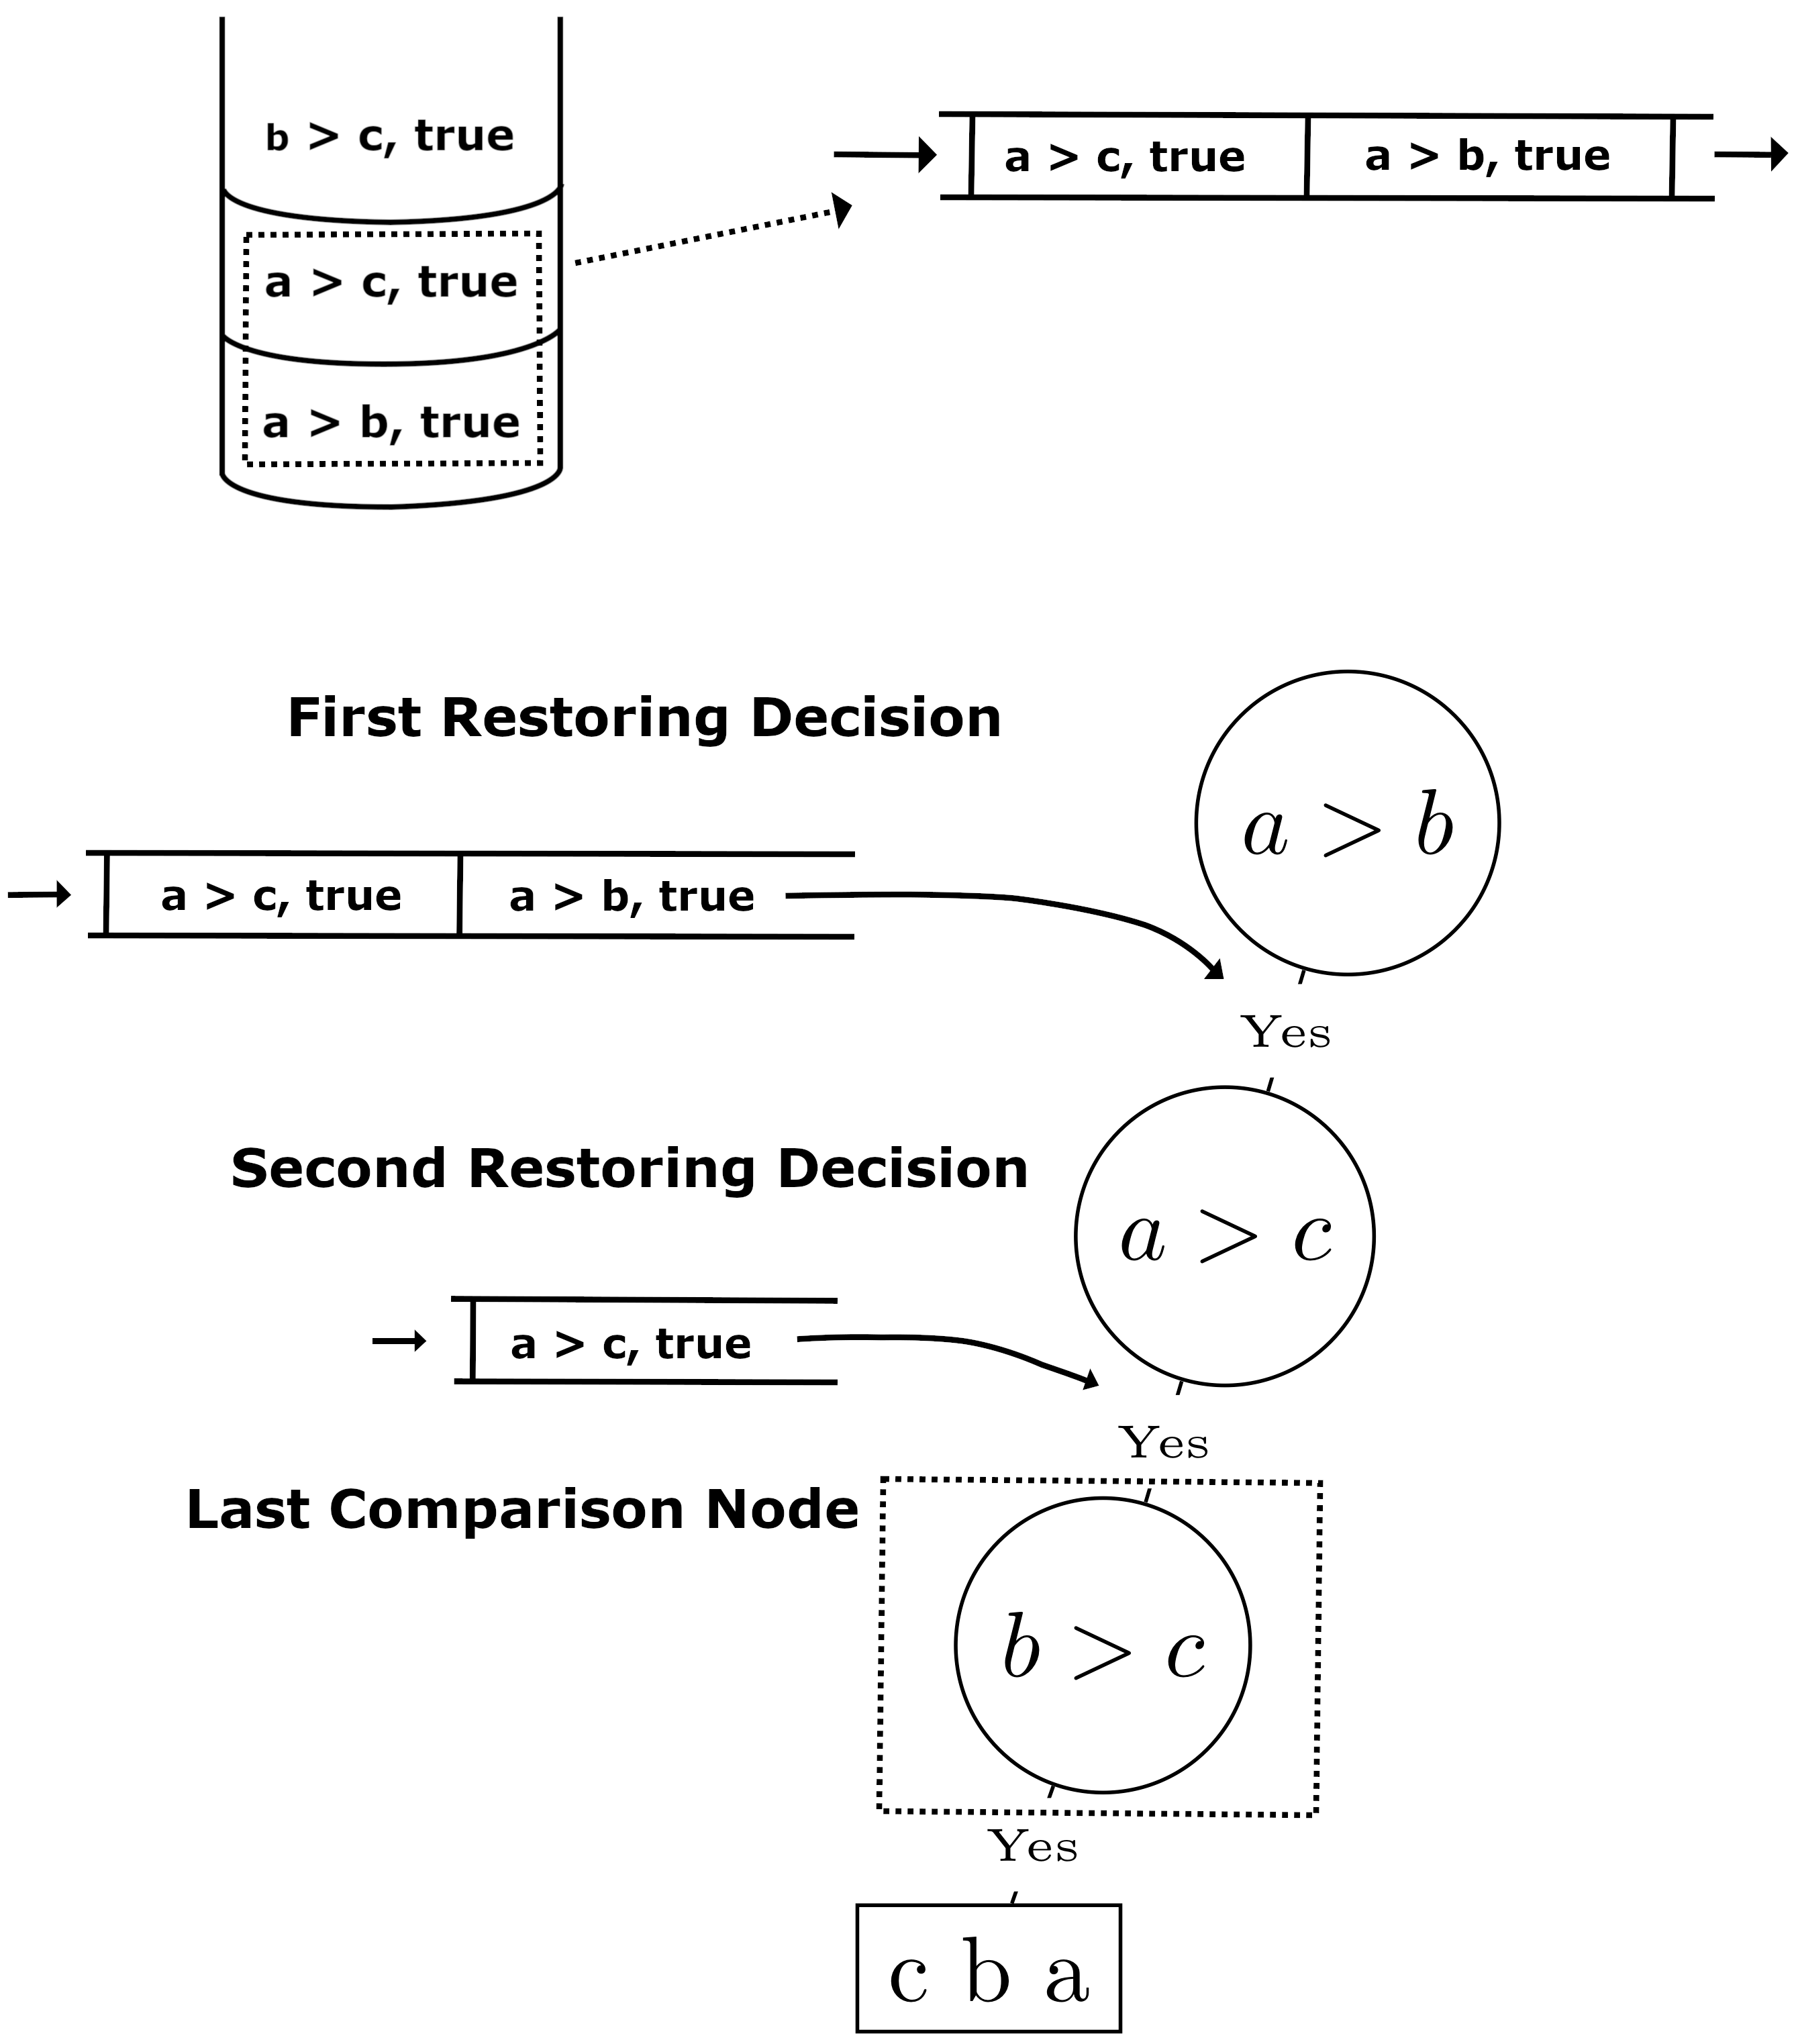
\includegraphics[width=0.8\linewidth]{figures/bubble_sort_step_2_formatted.png}
\caption{Analyzer Step 2 - Restoration Process}
\label{analyzer:2}
\end{figure}

%----------------------------------------------------------------------------------------

\end{column} % End of column 2.2

\begin{column}{\onecolwidmid} % The third column within column 2 (column 2.3)

%----------------------------------------------------------------------------------------
%	ANALYZER STEP 3
%----------------------------------------------------------------------------------------

\begin{figure}
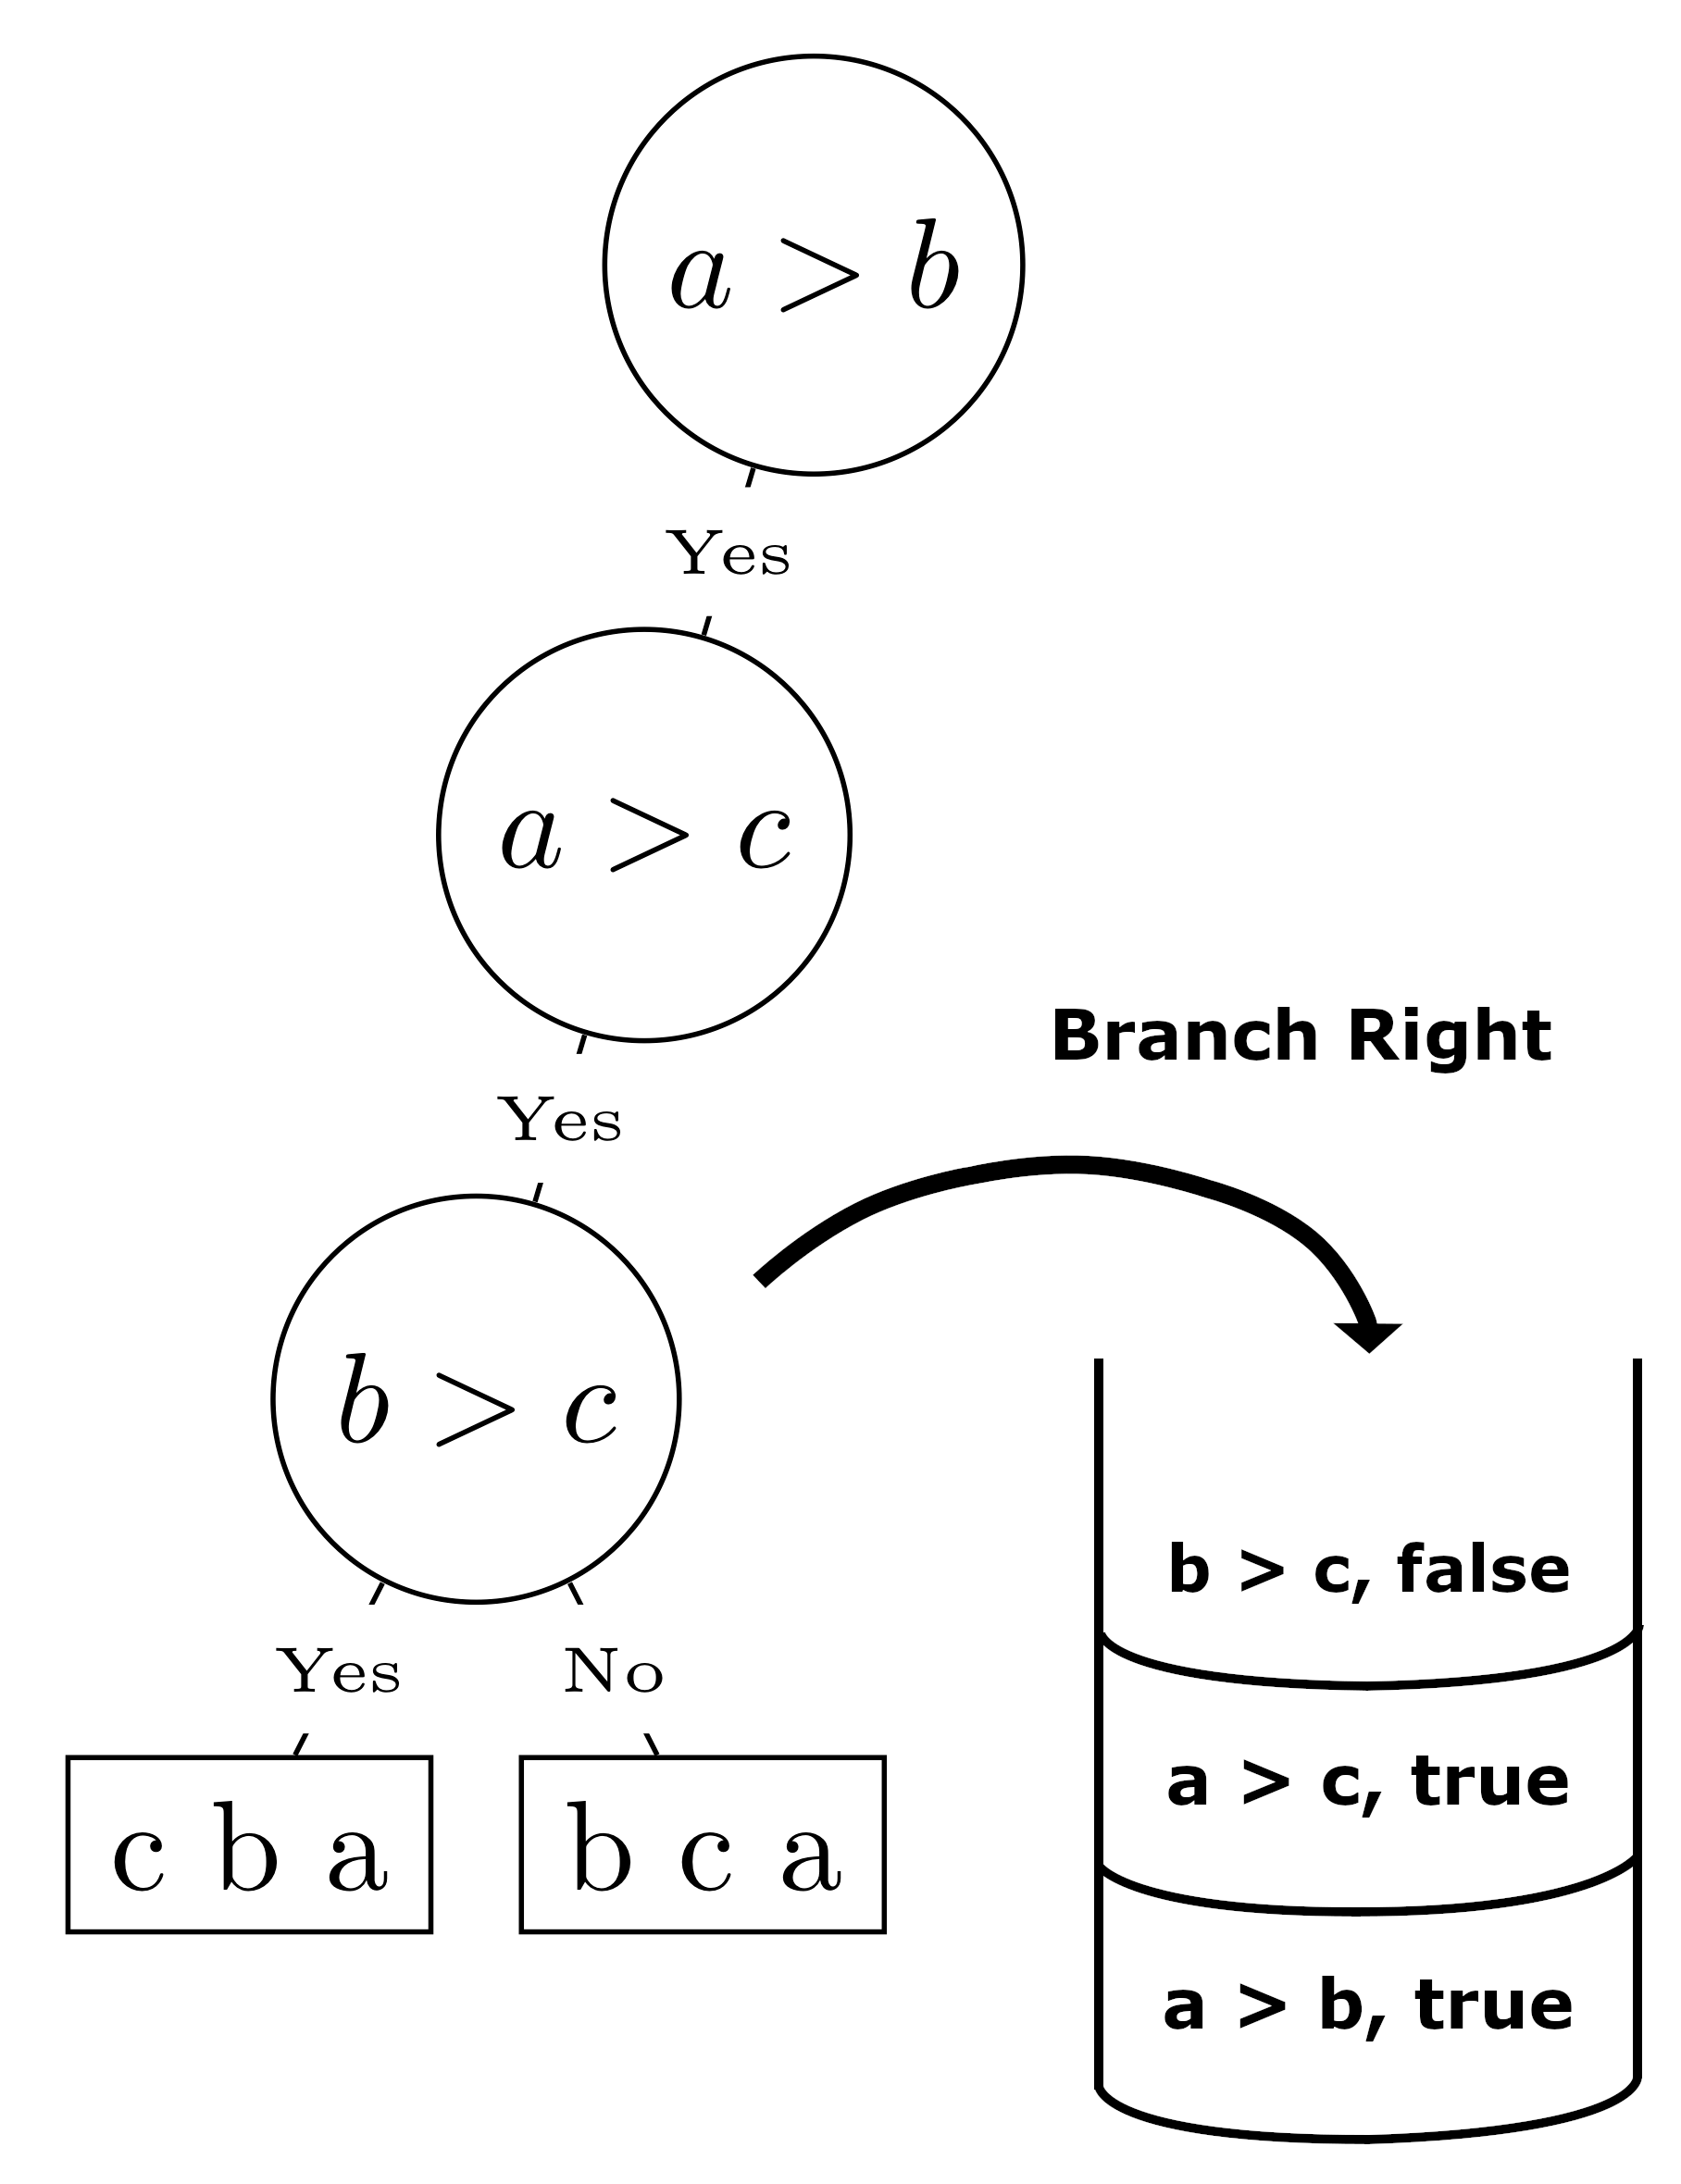
\includegraphics[width=0.8\linewidth]{figures/bubble_sort_step_3_formatted.png}
\caption{Analyzer Step 3 - Branching Right}
\label{analyzer:3}
\end{figure}

%----------------------------------------------------------------------------------------

\end{column} % End of column 2.3

\end{columns} % End of the split of column 2

\end{column} % End of the second column

\begin{column}{\sepwid}\end{column} % Empty spacer column

\begin{column}{\onecolwid} % The third column

%----------------------------------------------------------------------------------------
%	DECISION TREE GENERATOR
%----------------------------------------------------------------------------------------

\begin{block}{Decision Tree Generator}

To solve these problems, I designed an automatic analysis code library, the \textit{\textbf{Decision
Tree Generator}}. This library can take a modified version of any sorting algorithm and generate a
pruned-valid decision tree for some arbitrary input variables. To build the tree, the generator must
run the sorting algorithm through various situations, observing and controlling its comparisons of
records.

\end{block}

%----------------------------------------------------------------------------------------
%	GENERATOR FUNCTIONALITY
%----------------------------------------------------------------------------------------

\begin{block}{Generator Functionality}

Below is a description of one key functionality of the generator: state restoration.

\begin{enumerate}
\item For each comparison of records, the generator takes the comparison and decision made and
	pushes them to the state stack. In this case, the generator always chooses the decision to be
	false. Figure \ref{analyzer:1}
\item Once the algorithm stops running, the generator must restore its execution state to the last
	\textit{true} decision made. It does this by pulling the prior decisions out of the state stack
	and places them in a restoration queue. Every time a comparison is made, the next queue entry is
	dequeued and used as the next decision until empty. Figure \ref{analyzer:2}
\item The generator then makes the \textit{false} decision at that node, branching right. The
	process repeats until the whole tree is traversed. Figure \ref{analyzer:3}
\end{enumerate}

\end{block}


%----------------------------------------------------------------------------------------
%	CONCLUSION
%----------------------------------------------------------------------------------------

\begin{block}{Conclusion}

Visual analysis is key to designing efficient algorithms. The \textit{Decision Tree Generator} is
just the beginning of visual algorithm analysis programs that could be implemented to analyze other
types of algorithms in many different ways.

\end{block}

%----------------------------------------------------------------------------------------
%	REFERENCES
%----------------------------------------------------------------------------------------

\begin{block}{References}

\nocite{*} % Insert publications even if they are not cited in the poster
\small{\bibliographystyle{unsrt}
\bibliography{sample}\vspace{0.75in}}

\end{block}

\end{column} % End of the third column

\end{columns} % End of all the columns in the poster

\end{frame} % End of the enclosing frame

\end{document}
